\chapter{Concept}
\label{ch:concept}
This chapter introduces the functional and non-functional requirements of two 
applications - the container runtime and the benchmarking tool. 
In addition, architectural diagrams are provided and discussed. 
Example usage of both applications is shown.
This chapter also contains a thorough justification of the workloads deployed by the benchmarking tool as
well as the variables used to measure the performance of the sandboxed workloads.

\section{Container runtime}
The container runtime is the component responsible for wrapping a user-defined binary 
in a sandbox. It will be used by the benchmarking tool to wrap workloads in sandboxes.

\subsection{Functional requirements}
The Open Containers Initiative standardises the operations \cite{oci-runtime-operations} that 
a container runtime needs to support.

\begin{enumerate}[i]
\item The container runtime must provide clients with state information for a container
given its unique identifier. 
\label{requirements:container-runtime/1}
\item The container runtime must provide clients with the ability to create a new container. 
Users must supply the runtime with a unique identifier for the container and a path to a 
container bundle. The latter consists of a root filesystem and a configuration file that 
defines, amongst other things, the path to the user-defined binary and the set of namespaces
it will reside in.
\label{requirements:container-runtime/2}
\item The container runtime must provide clients with the ability to start a container. 
Users must provide the unique identifier of the container to start. 
This operation must execute the user-defined binary in the sandboxed environment.
\label{requirements:container-runtime/3}
\item The container runtime must allow users to kill the container process.
Users are required to provide the unique identifier of the container and the signal to be sent 
to the container.
\label{requirements:container-runtime/4}
\item The container runtime must allow users to delete the container.
The delete operation must remove all resources allocated in (\ref{requirements:container-runtime/2})
\label{requirements:container-runtime/5}
\item The container runtime must allow external applications to hook into well-defined points 
of a container's lifecycle.
\label{requirements:container-runtime/6}
\end{enumerate}

It is important to note that the container runtime's only responsibility is to sandbox processes. 
An external application, such as the benchmarking tool discussed later, 
must have the ability to interact with the runtime for the purpose of configuring 
the sandboxed environment. This includes operations such as creating network topologies that interconnect 
different containers or allocating shared filesystems. From this, requirement 
(\ref{requirements:container-runtime/6}) has been derived. 

\subsection{Non-functional requirements}
All requirements specified in this section are ranked in order of importance. 
\begin{enumerate}[i]
\item The container runtime must not pollute or damage the host system via its operation.
The runtime manages sensible resources, such as mount points and devices. It must in no way 
cause side effects on the host, leading to operational failure. This is also an important factor 
for allowing reproducibility of the work. Users must be able to use the runtime without fear of 
damaging their system. 
\label{requirements:non-functional/container-runtime/1}
\item The container runtime must support unprivileged containers, i.e containers that run without 
root privileges on the host system. This is in and of itself a functional requirement for running 
containers in multitenant environments. 
\label{requirements:non-functional/container-runtime/2} 
\item The container runtime must be implemented in a programming language with manual memory management.
Satisfying this requirement will ensure that future work aimed at measuring container boot times 
will not be hindered by unpredictable perturbations introduced by a garbage collector.
\label{requirements:non-functional/container-runtime/3}
\item The container runtime must consist of a library component and an executable component. 
This will allow users to implement their own abstractions on top of the library for other research-related 
purposes. 
\end{enumerate}

\subsection{Architecture}
\begin{figure}[H]
    \centering
    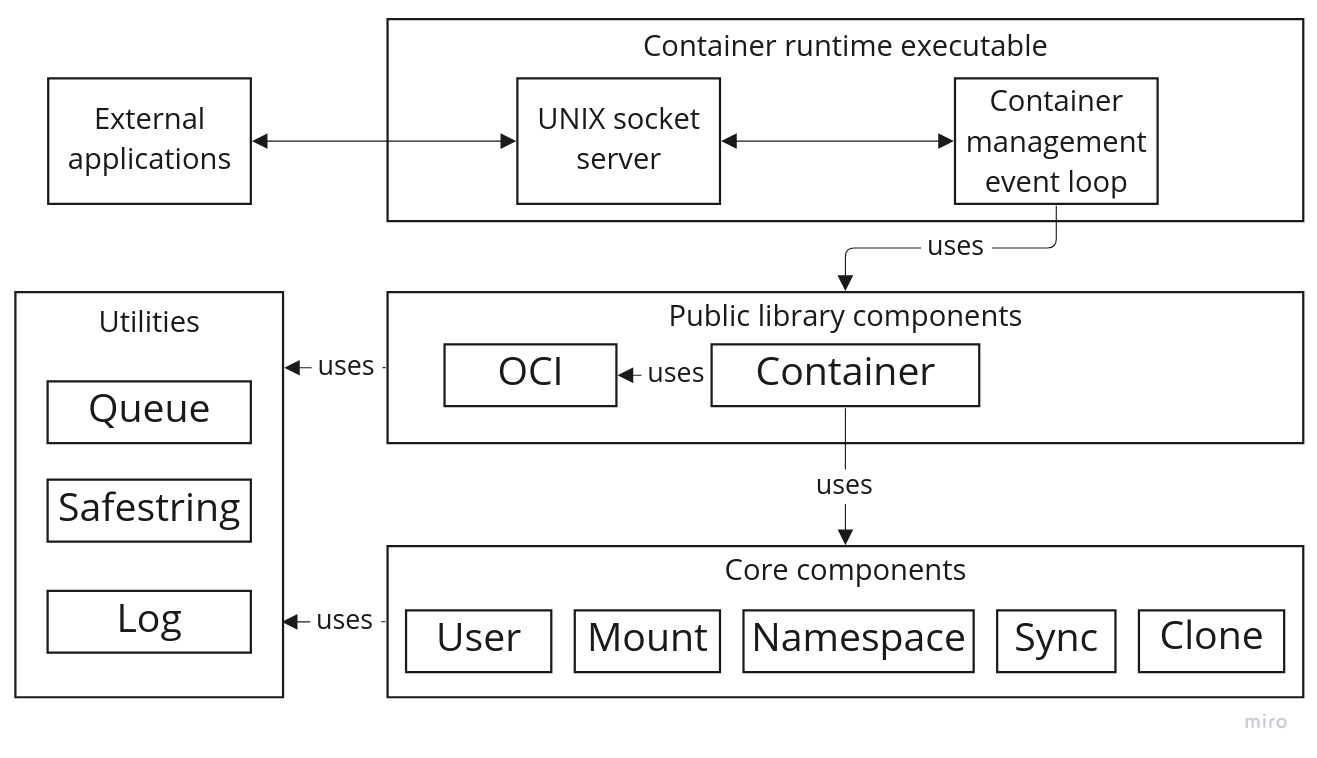
\includegraphics[width=0.55\textwidth]{images/concept/runtime-arch-overview.jpg}
    \caption{High-level overview of the runtime architecture}
    \label{images:concept/runtime-arch-overview.jpg}
\end{figure}
The architecture of the runtime is shown in Figure \ref{images:concept/runtime-arch-overview.jpg}.
It consists of a library and an executable that uses it to provide container 
management services to external applications. The library is split into three parts - utilities,
core components and public components. 

The utilities provide common data structures such as 
linked lists and queues. They also contain procedures for safe string manipulation, a logger,
and a multitude of helper macros that enable the safe management of resources such as file descriptors 
and heap memory. The core components directly interface with the kernel. 
They are responsible for configuring the container, 
i.e the execution environment of the user-defined application. On top, the public library 
components use the core components to provide a 
simple interface for creating, starting, killing and deleting containers. A container 
is represented as an opaque pointer and is only allowed to be accessed through library functions.

The runtime executable uses the container component to create and manage an in-memory queue 
of containers. Furthermore, an additional thread implements an event loop that monitors state changes of all containers 
in the run queue and reaps their resident processes to avoid leaking identifiers.
The main thread of execution implements a UNIX socket server that accepts requests
from external applications, e.g the benchmark tool, to satisfy the functional requirements
defined in the previous paragraph.

When a process is detached into a new user namespace, it's real user identifier is replaced by the kernel 
with the overflow identifier, also known as the \textit{nobody} user, which has no access to 
file objects that are not world readable and writable. 
For this reason, the container runtime must map a range of user identifers from the root user namespace 
into a range of user identifiers in the user namespace of the process. The user component in Figure 
\ref{images:concept/runtime-arch-overview.jpg} is responsible for this functionality. 

\begin{figure}[H]
    \centering
    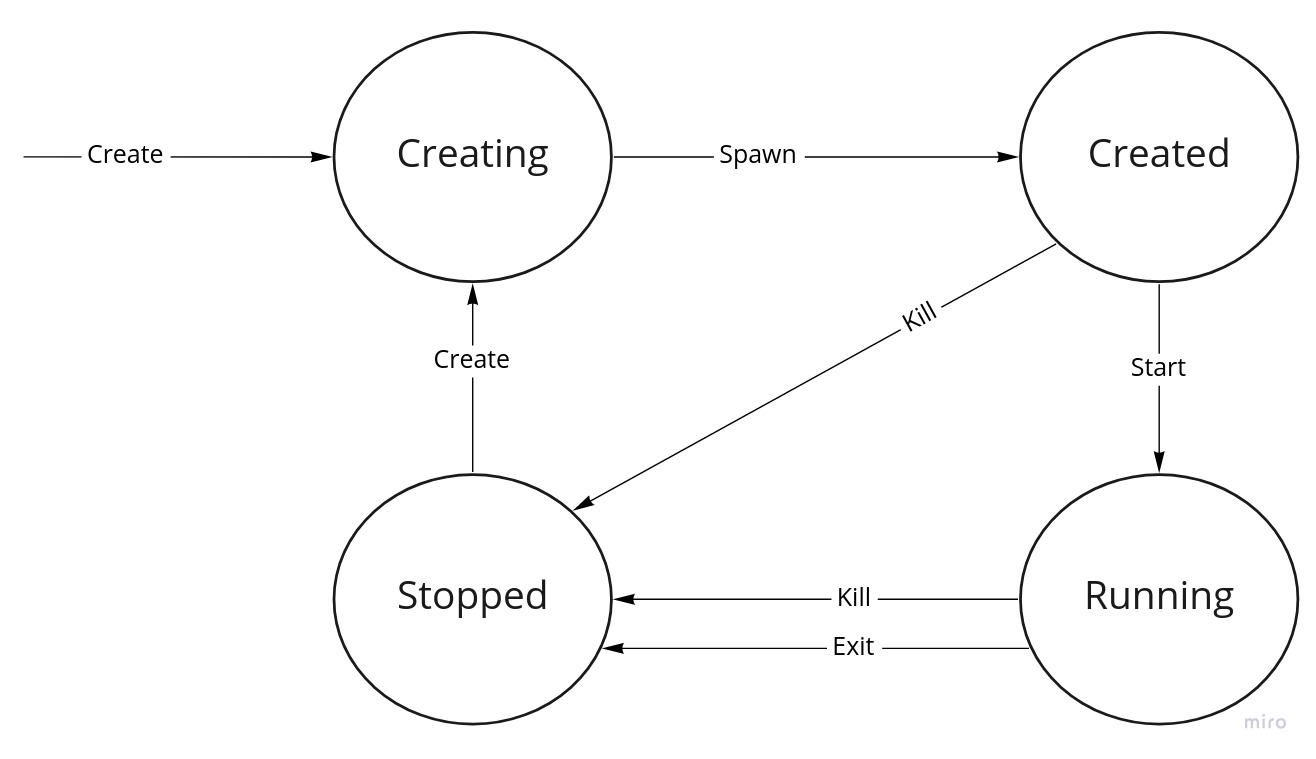
\includegraphics[width=0.5\textwidth]{images/concept/container-state-diagram.jpg}
    \caption{State transition diagram of container states. Every state transition is triggered by an operation, whose name is 
    specified in the arrow.}
    \label{images:concept/container-state-diagram.jpg}
\end{figure}

%\begin{table}[h!]
%    \centering
%    \begin{tabular}{ |m{3.5cm}|m{3.5cm}|m{20em}| }
%        \hline
%        Lifecycle Checkpoint & Request & Description \\
%        \hline
%        Runtime Creation & \verb|EVENT_RT_CREATE| & The container instructs the runtime to execute the runtime creation hooks on the host \\
%        \hline 
%        Container Creation & \verb|EVENT_CONT_CREATE| & The runtime instructs the container to execute the container creation hooks inside the container environment, after the runtime has been created \\
%        \hline 
%        Container Starting & \verb|EVENT_CONT_START| & The runtime instructs the container to execute the container start hooks inside the container environment, right before the user-defined binary is executed \\
%        \hline 
%        Container Started & \verb|EVENT_CONT_STARTED| & The container instructs the runtime to execute the container post-start hooks inside the runtime environment, right after the user-defined binary is executed \\
%        \hline 
%    \end{tabular}
%    \caption{Table of requests}
%    \label{table:concept/container-runtime/architecture/events}
%\end{table}

Every container has a dedicated root filesystem with its own set of device nodes,
pseudo filesystems, applications and libraries. The mount component in Figure \ref{images:concept/runtime-arch-overview.jpg}
atomically changes the container's root mount to a user-defined directory that holds its new root file system.
It then creates private mount points for all necessary pseudo filesystems, e.g \verb|proc|, \verb|sys|, and \verb|mqueue|. 
In addition, this component creates private device nodes for the container such as \verb|/dev/null| and \verb|/dev/urandom|.

The namespace component simply wraps some of the namespace system calls and provides a 
mechanism to enumerate a contiguous sequence of namespaces.

The clone component wraps the raw \verb|clone3()| system call and the \verb|glibc| wrapper 
into a portable (at least for \verb|x86_64| and \verb|aarch64|) set of functions.

The Open Containers Initiative (OCI) component is responsible for parsing a JSON configuration 
file that defines the container's execution environment. Code snippet \ref{code:oci-config.json} 
is an example of such a file. In addition, this component provides a mechanism for executing an 
arbitrary program, called a hook, that receives the container's state through its standard input stream as a JSON string.
Hooks are provided by external applications as part of the JSON configuration file and are executed
when a container transitions into a new state. A container's state transition diagram is shown in 
Figure \ref{images:concept/container-state-diagram.jpg}. For each unique state transition, a set of hooks 
gets executed. This design is defined as part of the runtime specification \cite{oci-runtime-lifecycle}.   

The synchronisation component defines an inter-process communication mechanism between 
the container runtime and a container. The typical communication flow follows the request-response pattern - 
one end produces a request and blocks until the other end consumes it and produces a response.
However, to enable concurrent work, a peer can \enquote{fire} a message and forget about the response.
The requests and responses are simple numeric values with semantic meaning. 


%The Open Containers Initiative (OCI) component is responsible for parsing a JSON configuration 
%file that defines the container's execution environment. Code snippet \ref{code:oci-config.json} 
%is an example of such a file. In addition, this component provides a mechanism for executing an 
%arbitrary program, called a hook, that receives the container's state through its standard input stream as a JSON string.
%These hooks are 
%This mechanism will be used by external applications to hook into well-defined points of a 
%container's lifecycle.
%The runtime prevents the program from temporaly interfering with it by starting a 
%timer and killing the program if it does not complete when the timer expires.
%Note that the synchronisation component is tightly coupled to the hook execution process. 
%The container synchronises with the runtime at specific points of its lifecycle. At those points, 
%a set of hooks defined by the external application is executed. 

\begin{figure}[H]
    \centering
    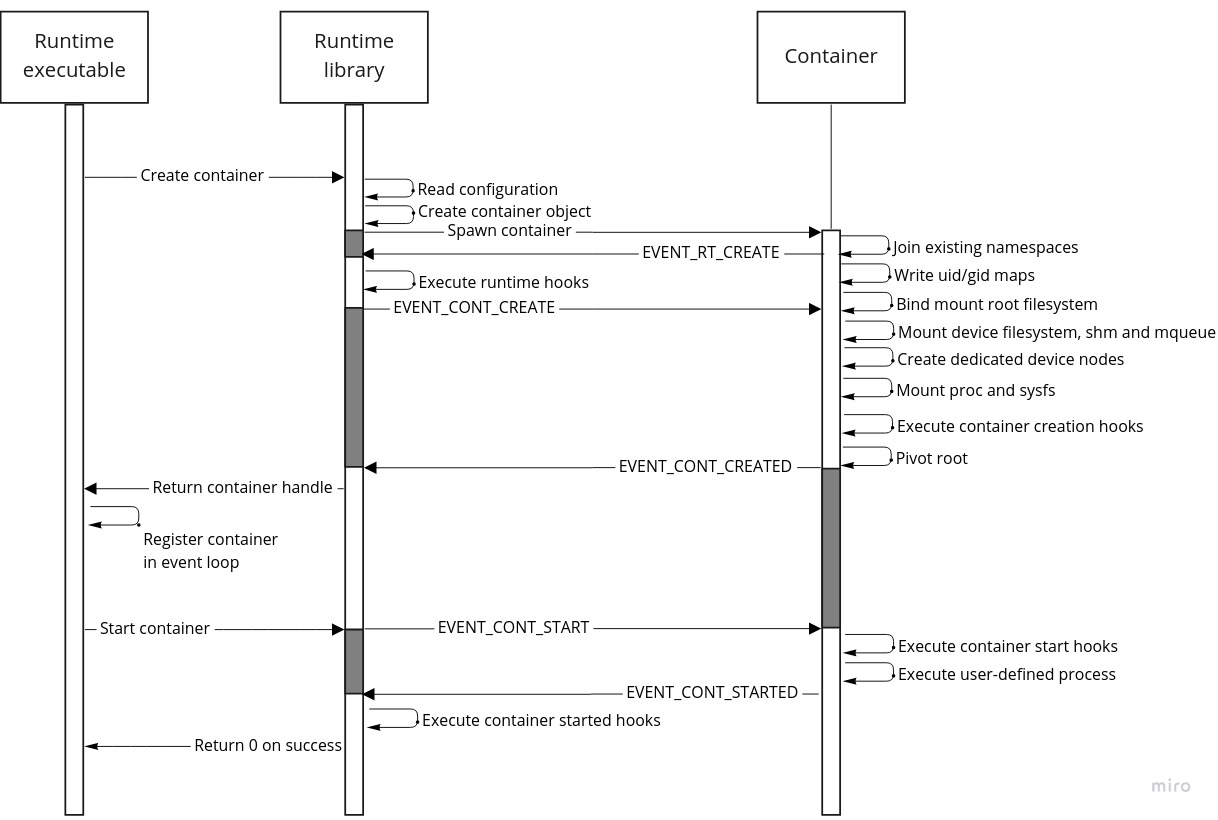
\includegraphics[width=0.8\textwidth]{images/concept/container-create-start-sequence-diagram.jpg}
    \caption{Sequence diagram highlighting the container creation and start operations}
    \label{images:concept/container-create-start-sequence-diagram.jpg}
\end{figure}

The container component brings all of the core components together. The sequence diagram in 
Figure \ref{images:concept/container-create-start-sequence-diagram.jpg} shows the procedures 
executed to create and start a container. The runtime executable invokes the create
operation, as defined in requirement (\ref{requirements:container-runtime/2}). 
The container component reads the configuration file and allocates 
an in-memory representation for the container. It then spawns the container process, which creates 
a freshly-allocated set of namespaces and joins already existing namespaces, depending on the namespace configuration 
specified in the file.
It then transitions into the \enquote{creating} state and notifies the runtime to execute the 
corresponding hooks by sending an \verb|EVENT_RT_CREATE| through the synchronisation component. 
The runtime receives the request, executes the runtime hooks, and notifies the child that it should transition 
into the \enquote{created} state by executing the container creation hooks and atomically swapping the old root mount 
with the new root filesystem. The container process then blocks indefinitely until it is killed 
or it receives a start request from the runtime executable. The latter will trigger yet another 
hook execution procedure, it will move the container into the \enquote{running} state and will afterwards run the user-defined binary. 
This is detected 
by the runtime, a set of post-start hooks is triggered, and the runtime executable is notified 
of the operation's completion.  

After the container is created, the executable is responsible for 
managing the container process. It does so by registering the container with an event loop that
polls container states and reaps processes that have terminated, which happens when the container 
transitions into the \enquote{stopped} state - either by exiting or being manually killed by the executable through 
a signal. 
\section{Benchmark}
Benchmarking is a tool to test performance in a controlled way, allowing different 
system and software configurations to be compared and analysed.

Our primary goal is to measure the overhead associated with isolating a process from the host system 


\subsection{Functional requirements}

\subsection{Non-functional requirements}
\begin{enumerate}[i]
    \item The benchmark must be repeatable to facilitate comparisons
    \label{requirements:non-functional/benchmark/1}
    \item The benchmark must be observable, either through visualisations or formatted text outputs, 
    so that it can be analysed
    \label{requirements:non-functional/benchmark/2}
    \end{enumerate}
\subsection{Methodology}

\subsection{Workloads}

\subsection{Command-line interface}